\documentclass[12pt]{article}

\usepackage[a4paper, margin=1in]{geometry}
\usepackage{graphicx}
\usepackage[absolute, overlay]{textpos}
\usepackage{fancyhdr}
\usepackage{siunitx}
\usepackage{tikz}
\usepackage{pgfplots}
\usetikzlibrary{decorations.pathmorphing}
\usetikzlibrary{math}
\usetikzlibrary{calc}

\pgfplotsset{compat=1.18}

\pagestyle{fancy} %for footers

\newcommand{\customsubject}{}   
\newcommand{\customtitle}{}

\newcounter{questionpartcounter}                  %Setup for question part counter for a,b,c listing
\renewcommand{\thequestionpartcounter}
{\alph{questionpartcounter}}

\newcounter{questionpartpartcounter}                  %Setup for question part  partcounter for a,b,c listing
\renewcommand{\thequestionpartpartcounter}
{\roman{questionpartcounter}}

\pagestyle{fancy} %for footers
\renewcommand{\headrulewidth}{0pt}
\fancyhf{}
\fancyfoot[R]{\thepage}

\newenvironment{worksheet}[2]
{
    
    \global\renewcommand{\customtitle}{#1}
    \global\renewcommand{\customsubject}{#2}


    \begin{textblock*}{5cm}(0.4cm,0.4cm)
   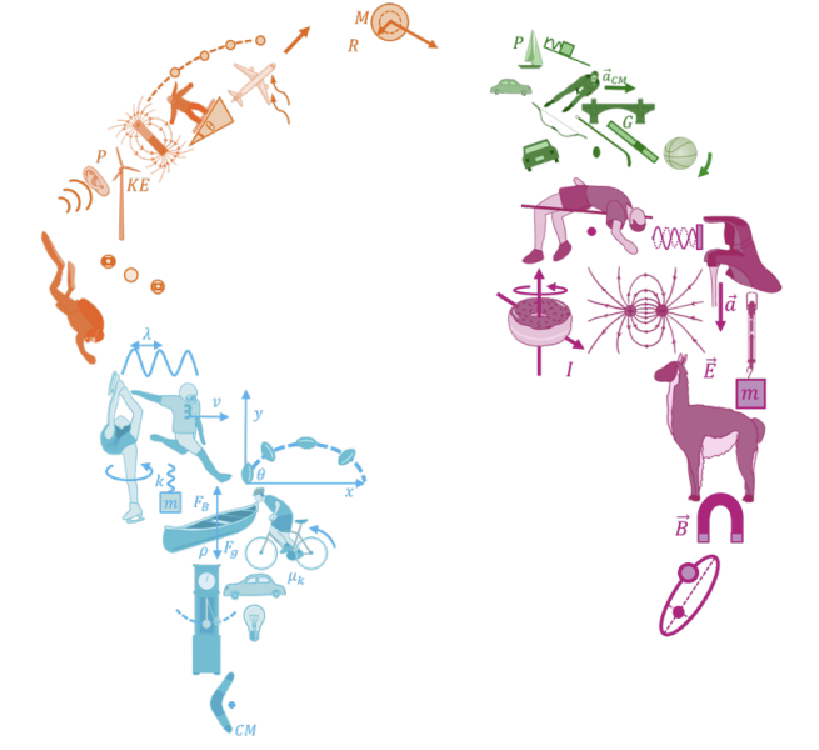
\includegraphics[width=4cm]{include/figures/bmdwlogo}
\end{textblock*}

    \vspace*{-1cm}
    
    {\large\textbf{\begin{center}\customtitle\end{center}}}

    \begin{center}\customsubject\end{center}
    
    \vspace{0.3cm}
    
    \hspace*{-1.5cm}\textbf{Name:\ \rule{4cm}{0.4pt}}\; 
    \textbf{Student \#: \ \rule{3cm}{0.4pt}}\;
    \textbf{Student Email \#: \ \rule{1.53cm}{0.4pt}}

    \vspace{0.5cm}

    
    \begin{enumerate}
}
{
    \end{enumerate}
   % \begin{textblock*}{10cm}(1cm, 28cm) {\footnotesize \scriptsize \customsubject}
    
%\end{textblock*}
}



\newcommand{\question}[2][1cm]{%
    \item
    \setcounter{questionpartcounter}{0}
    \setcounter{questionpartpartcounter}{0}
    {#2}
    \vspace{#1}
}

\newcommand{\questionpart}[2][1cm]{%
    \setcounter{questionpartpartcounter}{0}
    \stepcounter{questionpartcounter}
    (\thequestionpartcounter)~#2
    \vspace{#1}
}

\newcommand{\questionpartpart}[2][1cm]{%
      \stepcounter{questionpartpartcounter}
      \thequestionpartpartcounter.~#2
      \vspace{#1}
}

\newcommand{\operation}[1]{%
{\large $
#1
$}
}



\begin{document}

\begin{worksheet}{Physics Worksheet}{Newton's Laws}


\question[5.5cm]{Explain in your own words, how Newton would have theoretically arrived to the conclusion of the existance of a gravitational force from an apple having fallen on his head while sitting under an apple tree.}

\question[0cm]{Answer the following questions:}

\questionpart[3.5cm]{Is The Earth an inertial reference frame? Explain why or why not:}

\questionpart[3.5cm]{In what kind of situation could you approxomate The Earth to be an inertial reference frame?}

\questionpart[0cm]{What's a real world example where you cannot make this approxomation?}


\newpage


\question[0cm]{A block is held motionless between 2 walls}

\questionpart[0cm]{Make a free body diagram for the block and the left and right walls. Assume none of the surfaces are frictionless}

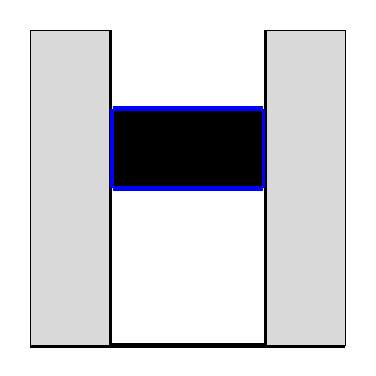
\begin{tikzpicture}[scale=1]
\scalebox{1.0}{
\draw[line width = 2pt] (0,0) -- (4,0);
\draw[line width = 2pt] (1,0) -- (1,4);
\draw[fill=gray!30] (0,0) rectangle (1,4);
\draw[line width = 2pt] (3,0) -- (3,4);
\draw[fill=gray!30] (3,0) rectangle (4,4);
\draw[line width = 2pt, color=blue] (1.05,3) -- (2.95,3);
\draw[line width = 2pt, color=blue] (1.05,2) -- (2.95,2);
\draw[line width = 2pt, color=blue] (1.05,2) -- (1.05,3);
\draw[line width = 2pt, color=blue] (2.95,2) -- (2.95,3);
\draw[fill=black] (1.07,2.03) rectangle (2.94,2.97);
}
\end{tikzpicture}
\vspace{2cm}

\questionpart[3cm]{Write Newton's Second Law for the block and the left and right walls} 


\question[0.25cm]{Below is a 2D cart with a vertical spring attached to a block. The cart also has 2 frictionless walls that hold the block motionless in the left and right directions relative to the cart. The system is currently at rest}


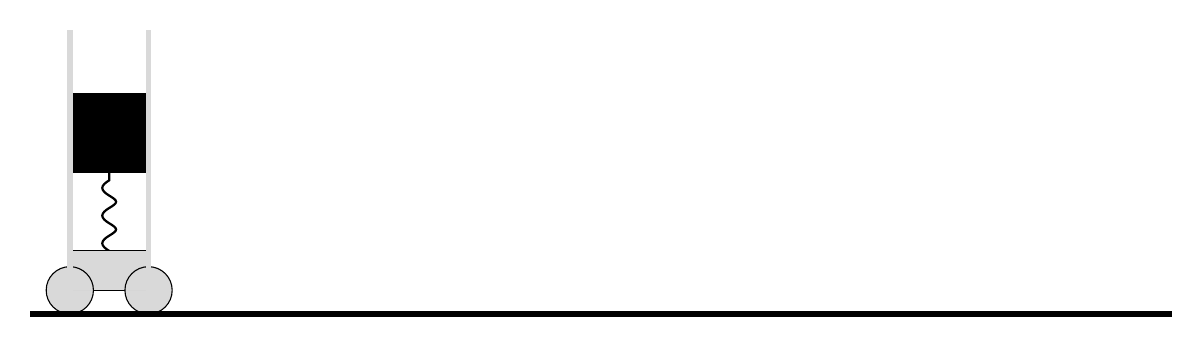
\begin{tikzpicture}
\scalebox{1.0}{
  \draw[fill=black] (0,0) rectangle (1,1);

  \draw[decorate, decoration={coil, aspect=0.1, segment length=10pt}, thick] (0.5,-1) -- (0.5,0);
\draw[fill=gray!30] (0,-1.5) rectangle (1,-1);

\draw[fill=gray!30, fill opacity=0.99] (0.0,-1.5) circle (0.3cm);
\draw[fill=gray!30, fill opacity=0.99] (1,-1.5) circle (0.3cm);

\draw[line width=2pt, color = gray!30] (0,-1.8)--(0, 1.8);
\draw[line width=2pt, color = gray!30] (1,-1.8)--(1, 1.8);
\draw[line width=2pt, color = black] (-0.5,-1.8)--(14, -1.8);
}

\end{tikzpicture}

\questionpart[0.25cm]{The cart is pushed to the right and the block is given an impulse in the downward direction both at $t = 0s$. Above, draw the theoretical trajectory of the block over time:}


\questionpart[0cm]{What simple function could describe the motion of the block $x(t)$?}

\end{worksheet}

\end{document}